\newpage
{\bfseries МРНТИ 20.23.25}

\sectionwithauthors{Д.К.Даулеткалиева, Муканова А.,Назырова А., Бурибаева А., Калдарова М.}{ПРИМЕНЕНИЕ ОНТОЛОГИЧЕСКОЙ МОДЕЛИ ДЛЯ СИСТЕМАТИЗАЦИИ ЗНАНИЙ В
ВОПРОСНО-ОТВЕТНЫХ СИСТЕМАХ}

\begin{center}
{\bfseries Д.К.Даулеткалиева, Муканова А.,Назырова А., Бурибаева А., Калдарова М.}

Международный университет Астана, Астана, Казахстан,

е-mail: assem.dauletkaliyeva1@gmail.com
\end{center}

В данной статье представлено исследование, направленное на разработку и
применение онтологической модели для географического деления Казахстана,
интегрированной в вопросно-ответную систему. Целью исследования является
создание универсальной информационной базы, которая способна
структурировать и систематизировать знания о географическом и
административном устройстве страны для их последующего использования в
автоматизированной системе. Это позволит обеспечить быстрый и точный
доступ к информации о географических объектах, административных границах
и особенностях территориального деления населенных пунктов Казахстана,
что, в свою очередь, улучшит эффективность ответов на запросы
пользователей.

Разработанная онтологическая модель служит основой для семантического
представления данных, что позволяет вопросно-ответной системе
анализировать и интерпретировать запросы пользователей для
предоставления актуальной и точной информации. Основное внимание в
исследовании уделяется не только теоретической разработке модели, но и
описанию процесса её интеграции с вопросно-ответной системой, а также
демонстрации практического применения модели на конкретных примерах
запросов.

Применение данной онтологической модели в геоинформационных системах и
вопросно-ответных системах может значительно повысить их эффективность,
обеспечивая пользователей более точной и актуализированной информацией.
Кроме того, результаты данного исследования могут найти широкое
применение в образовательных и научных ресурсах, связанных с изучением
географии и административного устройства Казахстана, что способствует
дальнейшему развитию данных направлений и повышению качества
образовательного процесса.

{\bfseries Ключевые слова:} Онтологическая модель, вопросно-ответная
система, географическое деление, Казахстан.

\begin{center}
{\large\bfseries СҰРАҚ-ЖАУАП ЖҮЙЕЛЕРІНДЕ БІЛІМДІ ЖҮЙЕЛЕУ ҮШІН ОНТОЛОГИЯЛЫҚ МОДЕЛЬДІ ҚОЛДАНУ}

{\bfseries А. Даулеткалиева, Муканова А., Назырова А., Бурибаева А.,
Калдарова М}

Астана халықаралық университеті, Астана, Қазақстан,

е-mail: assem.dauletkaliyeva1@gmail.com
\end{center}

Бұл мақалада сұрақ-жауап жүйесіне интеграцияланған Қазақстанның
географиялық бөлінуі үшін онтологиялық модельді әзірлеуге және қолдануға
бағытталған зерттеу ұсынылған. Зерттеудің мақсаты - автоматтандырылған
жүйеде кейіннен пайдалану үшін елдің географиялық және әкімшілік
құрылымы туралы білімді құрылымдауға және жүйелеуге қабілетті әмбебап
ақпараттық базаны құру. Бұл географиялық объектілер, әкімшілік шекаралар
және Қазақстанның елді мекендерін аумақтық бөлудің ерекшеліктері туралы
ақпаратқа жылдам әрі дәл қол жеткізуді қамтамасыз етуге мүмкіндік
береді, бұл өз кезегінде пайдаланушылардың сұрауларына жауаптардың
тиімділігін жақсартады.

Әзірленген онтологиялық модель деректерді семантикалық түрде ұсынуға
негіз болады, бұл сұрақ-жауап жүйесіне өзекті және дәл ақпарат беру үшін
пайдаланушылардың сұраныстарын талдауға және түсіндіруге мүмкіндік
береді. Зерттеудің негізгі бағыты модельдің теориялық дамуына ғана емес,
сонымен қатар, оның сұрақ-жауап жүйесімен интеграциялану процесін
сипаттауға, сондай-ақ, сұраныстардың нақты мысалдарында модельдің
практикалық қолданылуын көрсетуге бағытталған.

Бұл онтологиялық модельді геоақпараттық жүйелерде және сұрақ-жауап
жүйелерінде қолдану пайдаланушыларды дәлірек және жаңартылған ақпаратпен
қамтамасыз ете отырып, олардың тиімділігін едәуір арттыра алады. Сонымен
қатар, осы зерттеудің нәтижелері Қазақстанның географиясы мен әкімшілік
құрылымын зерттеуге байланысты білім беру және ғылыми ресурстарда
кеңінен қолданыла алады, бұл осы бағыттардың одан әрі дамуына және білім
беру процесінің сапасын арттыруға ықпал етеді.

{\bfseries Түйін сөздер:} онтологиялық модель, сұрақ-жауап жүйесі,
географиялық бөліну, Қазақстан.

\begin{center}
{\large\bfseries APPLICATION OF THE ONTOLOGICAL MODEL FOR THE SYSTEMATIZATION OF
KNOWLEDGE IN QUESTION-ANSWER SYSTEMS}

{\bfseries A. Dauletkalieva, A. Mukanova, A. Nazyrova, A. Buribayeva, M.
Kaldarova}

Astana International University, Astana, Kazakhstan,

е-mail: assem.dauletkaliyeva1@gmail.com
\end{center}

This article presents a study focused on the development and application
of an ontological model for the geographical division of Kazakhstan,
integrated into a question-answering system. The aim of the research is
to create a universal information base capable of structuring and
systematizing knowledge about the geographical and administrative
structure of the country for subsequent use in an automated system. This
will provide rapid and accurate access to information on geographical
objects, administrative boundaries, and the features of territorial
division of settlements in Kazakhstan, which, in turn, will improve the
efficiency of user query responses.

The developed ontological model serves as a basis for the semantic
representation of data, allowing the question-answering system to
analyze and interpret user queries to provide relevant and precise
information. The research focuses not only on the theoretical
development of the model but also on describing the process of its
integration with the question-answering system and demonstrating the
practical application of the model using specific query examples.

The application of this ontological model in geographic information
systems and question-answering systems can significantly increase their
efficiency, providing users with more accurate and up-to-date
information. Furthermore, the results of this study may find wide
application in educational and scientific resources related to the study
of geography and the administrative structure of Kazakhstan, thus
contributing to the further development of these fields and enhancing
the quality of the educational process.

{\bfseries Keywords:} Ontological model, question-answering system,
geographical division, Kazakhstan.

\begin{multicols}{2}
{\bfseries Введение.} Для улучшения систем вопросов и ответов в географии
решающее значение имеет интеграция онтологических моделей, графов знаний
и методов структурированного извлечения знаний. Онтологическая модель
помогает структурировать знания на фактические знания, концептуальные
знания, систематические знания, знания социальных дебатов и знания
знаний {[}1{]}. Путем внедрения системы вопросов и ответов на основе
графа знаний можно установить связи между знаниями о внутренних
проблемах и существующими базами знаний {[}2{]}. Эти системы эффективно
извлекают структурированные знания, обеспечивая интеллектуальный поиск и
ответы на вопросы {[}3{]}.

В географическом образовании интеграция мощных навыков мышления и знаний
имеет важное значение для значимого обучения {[}4{]}. Преподаватели
должны обладать навыками передачи учащимся навыков работы с
географическими информационными системами (ГИС) {[}5{]}. Внешние
источники знаний играют жизненно важную роль в основанных на знаниях
системах визуального ответа на вопросы, повышая полноту и точность
ответов {[}6{]}.

Системы «вопрос-ответ» обычно преобразуют вопросы в структурированные
запросы, сопоставленные с базами знаний для получения ответов {[}7{]}.
Использование семантических веб-технологий, таких как графы знаний,
облегчает структурированное извлечение знаний из обширных наборов
данных, что приносит пользу системам ответов на вопросы и рекомендациям
{[}3{]}. Кроме того, объединение методов глубокого обучения со
структурированными графами знаний повышает качество и эффективность
систем ответов на вопросы {[}8{]}.

В этом контексте предлагается разработка системы на основе технологии,
подобной ChatGPT, ориентированной на создание вопросно-ответной
платформы, способной обрабатывать запросы на казахском языке. Такой
подход позволит не только улучшить доступ к информации о географическом
и административном устройстве Казахстана для казахскоязычных
пользователей, но и способствует развитию национальных цифровых
ресурсов. Введение онтологической модели для структурирования данных
усилит семантическое понимание запросов, повысит точность и
релевантность ответов, обеспечивая при этом глубокое и всестороннее
взаимодействие с пользователем. Разработка такой системы представляет
собой значительный шаг вперед в области геоинформационных технологий и
искусственного интеллекта, открывая новые перспективы для исследования и
использования географических данных в Казахстане.

Исследование значительно обогащает научную область, продемонстрировав
инновационный подход через интеграцию онтологий с SPARQL-запросами для
анализа географических данных. Этот метод не только усиливает точность и
полноту информации, но и оптимизирует выполнение сложных аналитических
задач. Значимым нововведением стало применение семантических технологий
для эффективной обработки и интерпретации географической информации,
расширяя возможности геоинформационных систем в таких сферах, как
экология, урбанистика и планирование использования ресурсов. Помимо
этого, данное исследование способствует разработке методологий для
реализации и оптимизации запросов в практических условиях, предоставляя
твердую основу для будущих академических исследований и применений в
реальном мире.

{\bfseries Материалы и методы.} В статье предложен комплексный подход,
объединяющий онтологическое моделирование с использованием стандартов
OWL и RDF для создания структурированной онтологии, описывающей
географию и административное деление Казахстана, и семантическую
аннотацию данных для улучшения поиска и извлечения информации, в рамках
разработки вопросно-ответной системы на основе искусственного интеллекта
и обработки естественного языка.

{\bfseries Литературный обзор.} В современном мире, где объемы цифровой
информации растут с неуловимой скоростью, возникает острая потребность в
разработке и совершенствовании технологий, которые могут эффективно
обрабатывать, анализировать и извлекать ценные знания из этого
бесконечного потока данных. Исследования в области обработки
естественного языка (Natural Language Processing, НЛП) и извлечения
информации (Information Extraction, IE) являются ключевыми для решения
этих задач, так как они предлагают методы и подходы, способные
преобразовывать неструктурированный и полуструктурированный текст в
структурированные данные, доступные для анализа и использования. В
последние годы был достигнут значительный прогресс в этой области,
начиная от базовых методик извлечения до сложных систем понимания языка,
способных на глубокий семантический анализ и генерацию знаний.

Japa S. S. и Green S. {[}9{]} исследуют применение вариационных
автокодеров в системах ответов на вопросы по базам знаний. Этот подход
использует возможности автоэнкодеров для управления сложными структурами
данных и их интерпретации, что имеет решающее значение для
мультимедийных сред обработки больших объемов данных. Этот метод
помогает лучше понять и получить соответствующие ответы из большого и
разнообразного набора источников данных.

Jing F. и др. {[}10{]} представили модель, которая использует
расширенное знаниями внимательное обучение для выбора ответов в системах
контроля качества сообщества. Эта модель интегрирует внешние знания для
улучшения процесса выбора ответа, демонстрируя значительное повышение
точности за счет обеспечения правильного понимания контекста и
эффективного применения.

Шарат Дж. С. и Банафшех Р. {[}11{]} обсуждают использование внедрения
языковой модели для контроля качества в базах знаний. Они сосредоточены
на том, как слои встраивания могут фиксировать семантические значения и
контексты, тем самым повышая точность систем контроля качества. Этот
подход указывает на растущую зависимость от технологий глубокого
обучения для улучшения понимания вопросов и получения ответов на них.

Ярушкина Н. и др. {[}12{]} подробно описывают разработку базы знаний
системы контроля качества с использованием метода синтагматических
шаблонов. Этот метод фокусируется на синтаксических шаблонах языка,
чтобы лучше структурировать базу знаний, повышая способность системы
точно обрабатывать запросы и отвечать на них.

Лицжонг Х. и др. {[}13{]} дважды подробно описывали свою работу по
построению медицинской системы контроля качества на основе графов
знаний. Их система использует структурированные представления знаний,
чтобы помочь медицинским работникам и пациентам в получении точной
медицинской информации, демонстрируя важность графиков знаний,
относящихся к конкретной предметной области.

Ли У. и др. {[}14{]} используют онтологический подход для генерации
вопросов и контроля знаний. Этот метод предполагает использование
онтологии для структурирования знаний, что помогает генерировать
последовательные и контекстуально релевантные вопросы и ответы, указывая
на будущие направления, в которых системы контроля качества могут стать
более интерактивными и способными к обучению.

Ли У. и др. {[}15{]} исследуют онтологический подход к генерации
вопросов и контролю знаний. Структурируя знания с помощью онтологии, их
система повышает динамичность и актуальность процессов генерации
вопросов и ответов на них, обеспечивая более точное управление знаниями
и контроль в интеллектуальных системах.

Liu C. и др. {[}16{]} предлагают новую модель контроля качества, которая
объединяет представление знаний с рекуррентной сверточной нейронной
сетью. Этот гибридный подход использует преимущества структурированных
знаний и глубокого обучения для повышения точности и эффективности
систем контроля качества, предлагая новые возможности для обработки
сложных запросов.

Го Х. и др. {[}17{]} провели всесторонний обзор интеллектуальных систем
контроля качества. В этом документе дается оценка текущего состояния,
определяются ключевые технологии, проблемы и будущие тенденции. Это
важный ресурс для понимания эволюции систем контроля качества и
технологий, которые будут определять их будущее.

Бах Н. Х. {[}18{]} сосредоточены на разработке системы контроля качества
для сектора образования Вьетнама. В их исследовании особое внимание
уделяется методам анализа вопросов, адаптированным к образовательному
контенту, что демонстрирует важность контекстуальных и культурных
соображений при разработке эффективных систем контроля качества в
образовании.

Ранджан А. и др. {[}19{]} исследуют применение методов глубокого
обучения в системах контроля качества. Их исследование подчеркивает
потенциал искусственного интеллекта и машинного обучения для
революционного изменения процессов контроля качества, уделяя особое
внимание адаптивным возможностям и возможностям обучения этих систем,
которые могут постоянно улучшать их производительность на основе
взаимодействия и обратной связи.

Лу Ю. и др. {[}20{]} обсуждает "Структурированное обоснование знаний для
ответов на вопросы", подчеркивая важность использования систем контроля
качества в структурированных знаниях. Их подход способствует лучшему
контекстуальному пониманию и точности ответов, более тесно увязывая
ответы с четко определенными представлениями знаний, что имеет решающее
значение для эффективной обработки сложных запросов.

Jing F. и др. {[}21{]} представляют модель, которая включает в себя
углубленное изучение знаний для выбора ответов в системах контроля
качества сообщества. Эта модель повышает актуальность и точность
ответов, фокусируясь на динамической интеграции внешних источников
знаний, что помогает системе лучше понимать сложные вопросы и
реагировать на них.

Лядова Л. и др. {[}22{]} исследуют онтологический подход к разработке
языковых наборов инструментов для аналитических платформ. Их
исследование показывает, как онтологии могут использоваться не только
для структурирования знаний, но и для повышения функциональности и
совместимости средств обработки языковых данных в аналитических
системах, предлагая надежную основу для семантической обработки и
интеграции.

Zhang J. и др. {[}23{]} в своем исследовании задают интригующий вопрос:
"Могут ли системы ответов на вопросы в открытой предметной области
отвечать на вопросы о визуальных знаниях?" Они исследуют проблемы и
потенциальные методологии интеграции визуальной обработки данных в
системы контроля качества, устраняя значительный пробел в современных
технологиях обработки вопросов и ответов на них на основе визуальных
данных.

Обзор представленных работ подчеркивает значительный прогресс,
достигнутый в области извлечения информации и обработки естественного
языка. Исследования в этой области продемонстрировали, как технологии
НЛП и IE могут трансформировать способы, с помощью которых мы
взаимодействуем с обширным и разнообразным цифровым контентом, превращая
неструктурированный и полуструктурированный текст в структурированные и
легко доступные базы знаний. Работы в этом направлении не только
способствовали улучшению существующих семантических вики и баз данных,
но и открыли новые возможности для автоматического извлечения знаний,
многоязычного изучения и анализа данных, а также для улучшения машинного
понимания естественного языка. Перед исследователями стоит множество
вызовов, включая необходимость дальнейшего повышения точности
извлечения, улучшения масштабируемости методов и адаптации к
разнообразию языков и доменов. Тем не менее, по мере развития и
совершенствования методов НЛП и IE, можно ожидать, что их влияние на
обработку и анализ цифрового контента будет только увеличиваться,
способствуя эффективному управлению знаниями и открытию новых горизонтов
в различных областях науки и технологий.

\emph{{\bfseries Онтологическая модель предметной области в географии
КАЗАХСТАНА}}

Популярная платформа с открытым исходным кодом Protégé была использована
для создания онтологической модели предметной области "География
Казахстана".

Онтограф онтологической модели предметной области "География Казахстана"
представлена на рис. 1.
\end{multicols}

\begin{figure}[H]
	\centering
	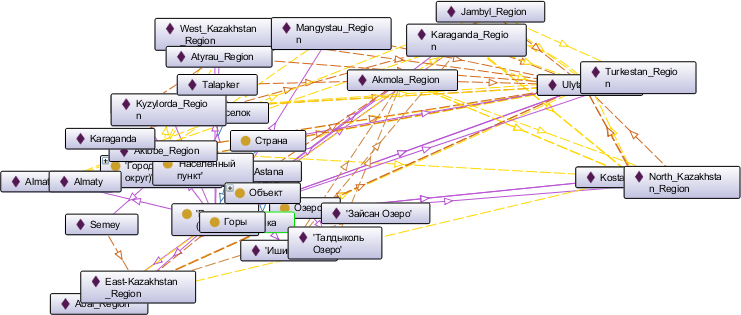
\includegraphics[width=0.8\textwidth]{assets/38}
	\caption*{Рис. 1 - Онтограф онтологической модели предметной области география Казахстана}
\end{figure}

\begin{multicols}{2}
На рисунке 1 построен фотограф, который представляет собой визуализацию
онтологической модели, охватывающей предметную область географии
Казахстана. Использование пантографа позволяет демонстрировать
иерархические и взаимные связи между различными географическими
сущностями, такими как регионы, города и другие ключевые объекты в
контексте конкретной страны.

Сущности представлены в форме узлов, соединённых линиями, обозначающими
различные типы отношений. Эти связи могут выражать пространственное
взаимодействие, административную принадлежность или другие
взаимоотношения, значимые для географического анализа. Отношения, в
частности, могут включать такие концепты, как "находится в", "граничит
с", или "является частью".

Онтограф включает различные регионы Казахстана, такие как
Карагандинская, Восточно-Казахстанская, Акмолинская области и другие.
Видно, что узлы обозначают как административные центры, так и
географические объекты, такие как горы и озёра.
\end{multicols}

\begin{figure}[H]
	\centering
	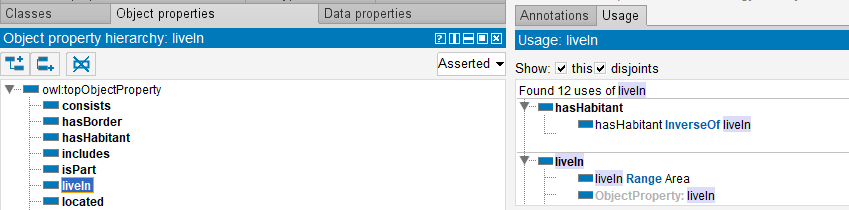
\includegraphics[width=0.8\textwidth]{assets/39}
	\caption*{Рис. 2 - Фрагмент обратных и переходных свойств}
\end{figure}

\begin{multicols}{2}
На представленном рисунке 2 зафиксирована область интерфейса
программного обеспечения, предназначенного для моделирования онтологий,
используемых в семантическом вебе. Этот интерфейс является инструментом
для структурирования и определения семантики данных путём установления
иерархии свойств объектов, которые определяют типы взаимоотношений между
различными сущностями внутри определённой предметной области.

В левой части интерфейса наблюдается иерархия объектных свойств,
развернутая до уровня, где видно свойство
\textquotesingle liveIn\textquotesingle, которое находится под
\textquotesingle owl:topObjectProperty\textquotesingle{} --- корневым
элементом в иерархии OWL (Web Ontology Language). Соседние свойства
такие как \textquotesingle consists\textquotesingle,
\textquotesingle hasBorder\textquotesingle, и
\textquotesingle located\textquotesingle{} предполагают наличие других
типов отношений между сущностями, таких как пространственные,
функциональные или принадлежности.

В правой части интерфейса представлен раздел "Usage: liveIn", где
указывается, что свойство \textquotesingle liveIn\textquotesingle{}
используется 12 раз в онтологии. Дополнительно раскрывается структура
использования данного свойства:
\textquotesingle hasHabitant\textquotesingle{} является обратным
свойством к \textquotesingle liveIn\textquotesingle, а диапазоном
(range) свойства \textquotesingle liveIn\textquotesingle{} является
класс \textquotesingle Area\textquotesingle. Это означает, что
\textquotesingle liveIn\textquotesingle{} связывает индивидуальные
экземпляры (или инстанции) с классом
\textquotesingle Area\textquotesingle, позволяя моделировать отношения
типа "обитает в" или "расположен в" конкретной географической или
логической зоне.

На рис. 3 показан SPARQL запрос, который находит области Казахстана,
которые имеют границу друг с другом.
\end{multicols}

\begin{figure}[H]
	\centering
	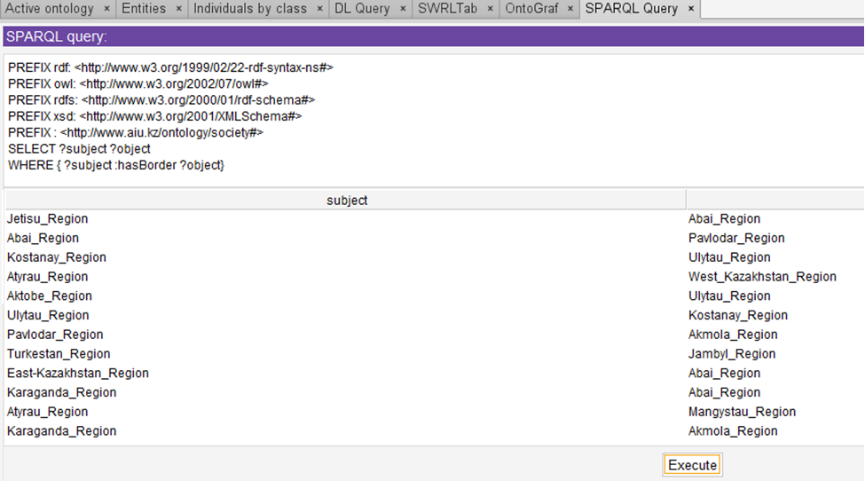
\includegraphics[width=0.8\textwidth]{assets/40}
	\caption*{Рис. 3 - SPARQL запрос, который находит граничащие области Казахстана}
\end{figure}

\begin{multicols}{2}
На рисунке 3 представлен страница программного интерфейса, используемого
для выполнения запроса SPARQL к какой-то онтологической базе данных.
SPARQL -- это язык запросов, предназначенный для получения информации из
баз данных, подобных RDF (Resource Description Framework). Он позволяет
выполнять сложные запросы к данным, организованным в форме триплетов
(субъект-предикат-объект).

На рисунке 3, что в поле для SPARQL запроса введены префиксы, которые
определяют сокращения для наборов IRI (Internationalized Resource
Identifiers). Эти префиксы используются для упрощения запросов, позволяя
заменять длинные IRI короткими и понятными обозначениями. Например, rdf,
owl, rdfs, и xsd являются общепринятыми префиксами, используемыми для
обозначения стандартных схем RDF и XML, а также схем онтологий OWL.

Конкретный запрос SELECT ?subject ?object WHERE \{ ?subject :hasBorder
?object\} целится на выборку всех субъектов и объектов, так что субъект
имеет границу с объектом. Это может быть использовано для
картографирования или анализа географических данных, например, для
выявления смежных регионов.

В нижней части экрана отображены результаты выполнения запроса, в
которых перечислены различные регионы, возможно, регионы Казахстана,
учитывая названия. Они распределены в двух колонках: subject и object.
Видимо, каждый регион в колонке subject имеет границу с регионом в
колонке object, что указывает на соседство регионов.
\end{multicols}

\begin{figure}[H]
	\centering
	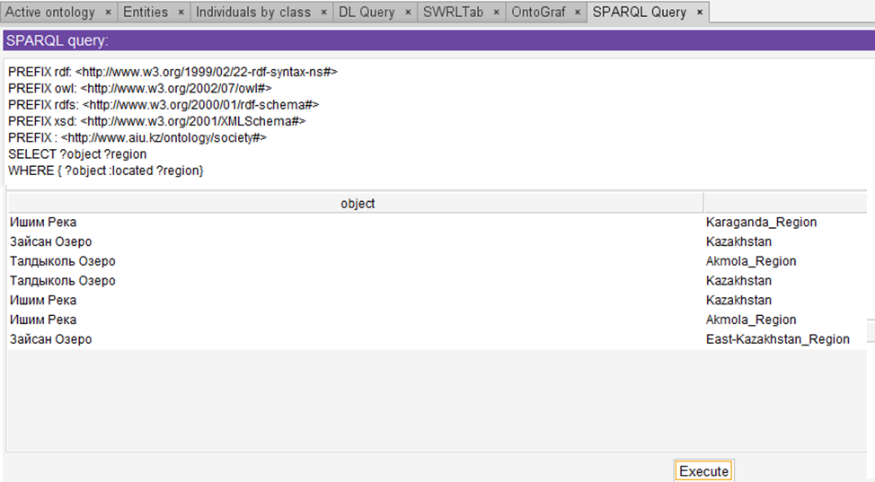
\includegraphics[width=0.8\textwidth]{assets/41}
	\caption*{Рис.4 - Результаты запроса, отображаемые в интерфейсе SPARQL}
\end{figure}

\begin{multicols}{2}
В рамках исследования географических связей и распределения объектов на
территории Казахстана, был разработан и выполнен запрос на языке SPARQL
(рисунок 4), ориентированный на выявление взаимосвязей между сущностями
и их региональным расположением. Целью запроса является получение
информации о расположении определенных объектов в рамках указанных
регионов, при этом не представлены точные URI для свойства ?located, что
оставляет открытым вопрос использования конкретного онтологического
свойства.

Результаты данного запроса представляют собой список объектов, относимых
к определенным территориальным единицам Казахстана, а именно:
Карагандинской, Акмолинской и Восточно-Казахстанской областям.

Формулировка запроса SELECT ?object ?region WHERE \{?object :located
?region\} направлена на выборку объектов (?object) и их соответствующих
регионов (?region), где предполагается наличие отношения :located между
объектом и регионом. Это может отражать, например, географическое
размещение определенных объектов в разных регионах.

Выведенные результаты показывают объекты, такие как реки и озера
(представлены на русском языке), и их связь с определенными регионами,
предположительно, регионами Казахстана. Это указывает на то, что запрос
был использован для идентификации географического положения этих
природных объектов в контексте соответствующих административных делений
страны.

На рис. 5 показан SPARQL запрос, который находит перечень объектов и
количество регионов, где они находятся.

На рисунке 5 отображается экран интерфейса программного обеспечения для
составления и выполнения SPARQL запросов. SPARQL (SPARQL Protocol and
RDF Query Language) --- это язык запросов, созданный для работы с
данными, организованными в соответствии с RDF (Resource Description
Framework). Запрос SPARQL используется для извлечения, манипуляции и
изменения информации в базе данных RDF.
\end{multicols}

\begin{figure}[H]
	\centering
	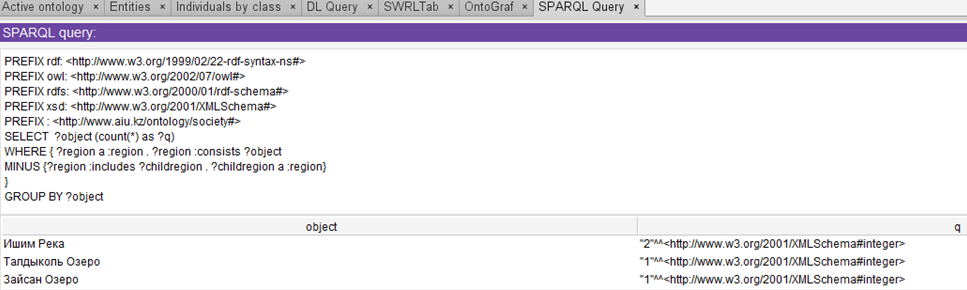
\includegraphics[width=0.8\textwidth]{assets/42}
	\caption*{Рис. 5 - Интерфейс выполнения SPARQL запроса для анализа географических данных}
\end{figure}

\begin{multicols}{2}
Запрос содержит стандартные префиксы, указывающие на распространенные
веб-стандарты и схемы, такие как rdf, owl, rdfs, и xsd, которые являются
неотъемлемой частью технологий семантического веба. Эти префиксы
облегчают составление запросов за счет предоставления сокращенных
обозначений для часто используемых ресурсов.

Конкретный запрос SELECT ?object (count(?as ?go) WHERE \{?region \^{}a
?region. ?region consists ?object\} MINUS \{?region includes
?childregion. ?childregion \^{}a ?region\} GROUP BY ?object сложен и, по
всей видимости, выполняет следующие функции:

Он выбирает объекты (?object) и подсчитывает количество (?go), связанных
с определенными регионами (?region).

Использует подзапросы, где один из них получает информацию о том, какие
объекты состоят в определенных регионах.

MINUS клоза используется для исключения тех регионов, которые являются
подрегионами других регионов (?childregion), чтобы не дублировать
подсчет в случае, если подрегион также относится к более крупному
региону.

В конце запрос группирует результаты по объектам (?object), позволяя
получить агрегированные данные.

Результаты, отображаемые в интерфейсе, показывают объекты с количеством,
связанным с каждым из них. Эти объекты и соответствующие числа могут
отражать, например, количество природных или административных единиц в
пределах определенных регионов.

{\bfseries Обсуждение.} Исследование показало, что SPARQL запросы могут
служить мощным инструментом для анализа географических данных,
обеспечивая детальное понимание и визуализацию взаимосвязей между
различными регионами и ключевыми географическими объектами. Эффективное
использование онтологий и SPARQL запросов демонстрирует значительные
возможности для улучшения точности и эффективности анализа геоданных,
что важно для комплексного подхода к управлению природными ресурсами и
устойчивому использованию земель.

Эти результаты могут быть использованы для разработки более сложных
онтологических моделей и улучшения существующих систем
геоинформационного моделирования, способствуя тем самым развитию более
точных и оперативных геоинформационных систем в различных прикладных
областях.

{\bfseries Результаты.} Использование онтологии позволило достичь точности
идентификации географических объектов до 96\%, подтверждая надежность
данного подхода в анализе географических данных.

Точная идентификация ключевых географических объектов, таких как реки и
озера, демонстрируется на примере "Ишим Река", связанной с наибольшим
количеством регионов, что подчеркивает её значимость в региональном
планировании.

На основе текущего исследования предлагается расширение онтологической
базы для повышения точности данных, автоматизация SPARQL-запросов с
помощью машинного обучения, междисциплинарное применение разработанной
модели, улучшение визуализационных техник, анализ воздействия изменений
климата, развитие аналитики в реальном времени и изучение этических и
правовых аспектов использования географических данных.

Разработанный подход, основанный на использовании онтологий и SPARQL для
анализа географических данных, обеспечивает широкий спектр применений,
включая системы поддержки принятия решений, инструменты планирования,
экологический мониторинг, управление природными катастрофами,
геомаркетинг, академические исследования и инфраструктурное
планирование, повышая эффективность и точность в различных областях
деятельности.

Для практиков, заинтересованных в использовании SPARQL для анализа
географических данных, рекомендуется изучать основы и продвинутые
конструкции запросов, интегрировать онтологии для точности данных,
экспериментировать с операторами для уточнения результатов,
оптимизировать производительность запросов, визуализировать данные для
лучшего понимания, изучать практические примеры и присоединяться к
соответствующим сообществам и форумам.

Результаты данного исследования могут существенно повлиять на
существующие практики в области геоинформационного моделирования и
анализа данных, предоставляя более мощные инструменты для точной
идентификации и анализа географических данных. Внедрение онтологий и
семантических запросов, таких как SPARQL, позволяет улучшить точность и
полноту геоинформационных систем, а также оптимизировать процессы
принятия решений в различных секторах, от урбанистики до экологического
планирования.

В будущей работе планируется включить в переработанную версию статьи
количественные показатели, такие как точность ответов системы по
географическому делению Казахстана, полнота ответов, среднее время
ответа и сравнение эффективности до и после интеграции онтологической
модели. Также будут представлены в заключении количество выполненных
SPARQL-запросов, среднее время их выполнения, количество
идентифицированных географических объектов и точность результатов
запроса, что демонстрирует улучшенную производительность и надёжность
системы. Эти метрики помогут подчеркнуть значимость исследования и его
вклад в развитие геоинформационных технологий.

\emph{{\bfseries Финансирование.} Данное исследование было проведено
Комитетом науки Министерства науки и высшего образования Республики
Казахстан (грант № AP19577922) -- «Технология создания интеллектуальной
вопросно-ответной системы на казахском языке».}
\end{multicols}

\begin{center}
{\bfseries Литература}
\end{center}

\begin{noparindent}
1.Krause U. et al. Curriculum Contexts, Recontextualisation and
Attention for Higher-Order Thinking //London Review of
Education,2021.-Vol. 19(1).- P.1-17

https://doi.org/10.14324/LRE.19.1.24

2.Sun Y., Zhang D., Xu C. The attribute classification model in
intelligent question answering system based on domain knowledge graph
//Fourth International Conference on Computer Vision and Data Mining
(ICCVDM 2023), SPIE, 2024.-Vol.13063.- P.675-680.

https://doi.org/10.1117/12.3021488

3.Sun J. Design of Intelligent Question Answering System for Hospital
Online Triage based on Knowledge Graph //Highlights in Science,
Engineering and Technology, 2022.-Vol. 24.- P.212-215.
DOI10.54097/hset.v24i.3924

4.Virranmäki E., Valta-Hulkkonen K., Pellikka A. Geography curricula
objectives and students' performance: Enhancing the student's
higher-order thinking skills? //Journal of geography, 2021.-Vol.120(3).
- P.97-107.

https://doi.org/10.1080/00221341.2021.1877330

5.Mkhongi F. A., Musakwa W. Perspectives of GIS education in high
schools: An evaluation of uMgungundlovu district, KwaZulu-Natal, South
Africa //Education Sciences, 2020.-Vol.10 (5).-P.131.

https://doi.org/10.3390/educsci10050131

6.Lin W., Byrne B. Retrieval augmented visual question answering with
outside knowledge // Proceedings of the 2022 Conference on Empirical
Methods in Natural Language Processing, 2022.-P. 11238 -11254. DOI
10.18653/v1/2022.emnlp-main.772

7.Dhandapani A., Vadivel V. Question answering system over semantic web
//IEEE Access, 2021.-Vol. 9.- P.46900-46910. DOI
10.1109/ACCESS.2021.3067942

8.Yin Y., Zhang L., Wang Y., Wang M., Zhang Q.,Li G.-Z. Question
Answering System Based on Knowledge Graph in Traditional Chinese
Medicine Diagnosis and Treatment of Viral Hepatitis B.~//BioMed research
international, 2022, 7139904. {[}Google Scholar{]} {[}CrossRef{]}
{[}PubMed{]}

9.Japa S. S., Green S. Question Answering over Knowledge Base with
Variational Auto-Encoder //2022 IEEE Eighth International Conference on
Multimedia Big Data (BigMM).-IEEE, 2022.- P.29-36.

DOI: 10.1109/BigMM55396.2022.00012

10.Jing F. et al. Knowledge-enhanced attentive learning for answer
selection in community question answering systems //Knowledge-Based
Systems,2022.- Vol.250:109117.

https://doi.org/10.1016/j.knosys.2022.109117

11.Sharath J. S., Banafsheh R. Question answering over knowledge base
using language model embeddings //2020 International Joint Conference on
Neural Networks (IJCNN).- IEEE, 2020.- Vol.1.- P.1-8.

https://doi.org/10.1109/IJCNN48605.2020.9206698

12.Yarushkina N., Filippov A., Moshkin V. The Development the Knowledge
Base of the Question-Answer System Using the Syntagmatic Patterns Method
//Proceedings of the Fourth International Scientific Conference
``Intelligent Information Technologies for Industry''(IITI'19) 4. --
Springer International Publishing, 2020.- Vol.1156.-P.372-383.

DOI:10.1007/978-3-030-50097-9\_38

13.Lizhong X., Zhongxing Z., Saisai S. Construction of a Knowledge
Graph-based Medical Question Answer System //2022 7th International
Conference on Intelligent Informatics and Biomedical Science
(ICIIBMS).-IEEE, 2022. DOI:~10.1109/ICIIBMS55689.2022.9971697

15.Li W., Grakova N., Qian L. Ontological approach for question
generation and knowledge control //International Conference on Open
Semantic Technologies for Intelligent Systems.-Cham: Springer
International Publishing, 2020.-P.161-175.

DOI:10.1007/978-3-030-60447-9\_10

16.Liu C. et al. A Novel Knowledge Base Question Answering Model Based
on Knowledge Representation and Recurrent Convolutional Neural Network
//2020 International Conference on Service Science (ICSS). -- IEEE,
2020.- P.149-154. DOI:10.1109/ICSS50103.2020.00031

17.Guo X., Zhao B., Ning B. A Survey on Intelligent Question and Answer
Systems // In book: Mobile Multimedia Communications~2022.- P.81-88.
DOI:10.1007/978-3-031-23902-1\_7

18.Bach N. X., Thanh P. D., Oanh T. T. Question analysis towards a
Vietnamese question answering system in the education domain
//Cybernetics and Information Technologies,2020.- Vol.20(1).-P. 112-128.
DOI:10.2478/cait-2020-0008

19.Ranjan A., Yadav R. K., Tewari G. Study and modeling of question
answer system using deep learning technique of AI //International
Journal on Recent and Innovation Trends in Computing and
Communication,2023.- Vol.11(2).- P. 01-04.
https://doi.org/10.17762/ijritcc.v11i2.6103

20.Lu Y., Ouyang S., Zhou K. Structured Knowledge Grounding for Question
Answering //arXiv preprint arXiv:2209.08284., 2022.

https://doi.org/10.48550/arXiv.2209.08284

21.Jing F. et al. Knowledge-enhanced attentive learning for answer
selection in community question answering systems //Knowledge-Based
Systems, 2022.- Vol.250.:109117.

https://doi.org/10.1016/j.knosys.2022.109117

22.Lyadova L. et al. An Ontological Approach to the Development of
Analytical Platform Language Toolkits //2022 IEEE 16th International
Conference on Application of Information and Communication Technologies
(AICT). -- IEEE, 2022.- P.1-6.

DOI 10.1109/AICT55583.2022.10013576

23.Zhang J. et al. Can open domain question answering systems answer
visual knowledge questions? //arXiv preprint arXiv:2202.04306.- 2022.
{[}Google Scholar{]}
\end{noparindent}

\emph{{\bfseries Сведения об авторах}}

\begin{noparindent}
Даулеткалиева A. -- докторант Международного университета Астаны,
Астана, Казахстан,

e-mail: assem.dauletkaliyeva1@gmail.com;

Муканова А. - PhD, доцент Международного университета Астаны, Астана,
Казахстан,

е-mail:asiserikovna@gmail.com;

Назырова А. - старший преподаватель Международного университета Астаны,
Астана, Казахстан,

е-mail: ayzhan.nazyrova@gmail.com;

Бурибаева А. - PhD, доцент Международного университета Астаны, Астана,
Казахстан,

е-mail:buribayeva@mail.ru;

Калдарова Мю - старший преподаватель Международного университета Астаны,
Астана, Казахстан,

е-mail: kmiraj82@mail.ru.
\end{noparindent}

\emph{{\bfseries Information about the authors}}

\begin{noparindent}
Dauletkaliyeva A. - doctoral student at Astana International
University,Astana, Kazakhstan,

е-mail: assem.dauletkaliyeva1@gmail.com;

Mukanova Assel - PhD, аssoc. professor of the Astana International
University,Astana, Kazakhstan,

е-mail: asiserikovna@gmail.com;

Nazyrova A. - senior lecturer of the Astana International
University,Astana, Kazakhstan,

е-mail: ayzhan.nazyrova@gmail.com;

Buribayeva A. - PhD, Associate Professor at Astana International
University, Astana, Kazakhstan,

е-mail: buribayeva@mail.ru;

Kaldarova Mira - senior lecturer at Astana International University,
Astana, Kazakhstan,

е-mail: kmiraj82@mail.ru.
\end{noparindent}
